% ------------------------------------------------------
\chapter{Fejlesztői dokumentáció}
\label{ch:developer}
% ------------------------------------------------------



% ------------------------------------------------------
\chapter{Szimulációs eredmények}
% ------------------------------------------------------

GPU környezetben nehéz algoritmusokat tesztelni és hibákat javítani, a masszívan párhuzamos környezet miatt, ezért az algoritmusokat egy szálon, Matlabban is implementáltam. A vizsgálat középpontjában az algoritmusok stabilitása és konvergenciája állt. 

\section{Gradiens módszerek stabil paraméterezése}

A gradiens módszer egyszerűsége ellenére meglepően jól teljesít Bézier felületeken abban az esetben, ha a tanulási rárát ($\alpha$) a lehető legnagyobb értékre állítjuk. Ekkor azonban nem tudunk garantálni semmiféle konvergenciát. Emiatt olyan hiperparaméter-beállítást keresünk, mely szélsőséges esetben is a lokális minimumhoz konvergál.

\subsection{Rosenbrock-függvény}
A Rosenbrock-függvény egy klasszikus "nehéz" példa, melyet optimalizációs algoritmusok tesztelésére szoktak alkalmazni. Definíciója:
$$ f(x,y) = (a-x)^2 + b(y-x^2)^2 $$
Ennek a globális minimuma az $(a,a^2)$ helyen van. Az $a$ paraméter értéke általában $1$. A $b$ paraméterrel a probléma ,,nehézségét'' lehet állítani. Minél nagyobb a $b$ érték, annál nagyobb lesz a gradiensvektor hossza. Én $20$-ra állítottam.
\begin{figure}[H]
	\centering
	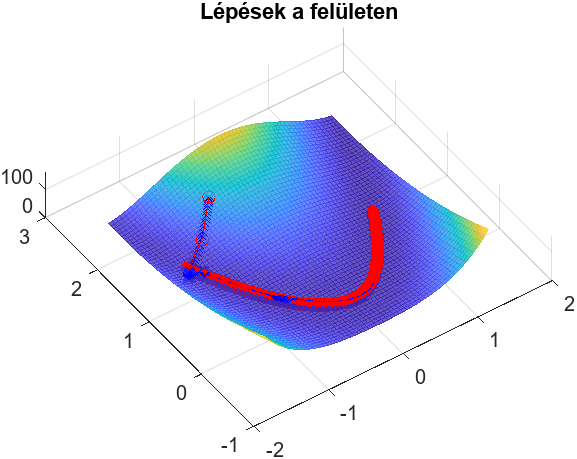
\includegraphics[width=0.4\textwidth]{RB_surf}
	\hspace{5pt}
	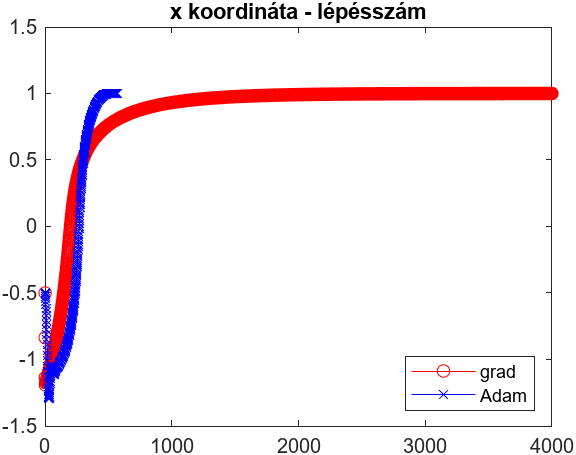
\includegraphics[width=0.4\textwidth]{RB_x}
	\caption{Stabil paraméterezés a Rosenbrock függvényen}
	\label{fig:RB}
\end{figure}
A gradiens módszer paramétere: $\alpha = 0,005$ \\
Az AdaMax módszer paraméterei: $\alpha = 0,005$, $\beta_1 = 0,9$, $\beta_2 = 0,99$ \\
\Aref{fig:RB} ábrán pirossal a gradiens módszer lépéseit, kékkel az AdaMax módszer lépéseit jelöltem. Az AdaMax módszer $569$ lépésben $10^{-6}$ nagyságrendű hibával konvergál. A gradiens módszer hibája $1000$ lépés után $1/10$-nél nagyobb, és még $5000$ lépés után is $10^{-4}$ nagyságrandű.

Ebből a példából jól látszik a bonyolultabb módszer előnye, ha megköveteljük a konvergenciát nehezebb példákra is.



\section{Globális minimum harmadfokú Bézier-felületen}

A módszereket Bézier-felületeken is összehasonlítottam. A cél alapvetően a Bézier-felület távolságfüggvényének generálása. Ehhez a globális minimumot kell meghatározni. Ezt úgy kívánjuk elérni, hogy a lokális optimumkereső algoritmust több pontból elindítjuk. Az itt következő példák intuíciót adnak az indítási pontok minimális számára, amit a következő részben szimulációval validálok.

\subsection{Sarokpontok}
\Aref{fig:corners} példában az látszik, hogy lokális optimum közel lehet a felület sarkához ($(0,0),(0,1),(1,0),(1,1)$ pontok). Ha a felület belsejéhez tartozó kontrolpontok koordinátáit nagyobbra állítjuk, a baloldali ábrán látható lokális szélsőértékek tetszőlegesen közel kerülhetnek a sarokpontokhoz. 
\begin{figure}[H]
	\centering
	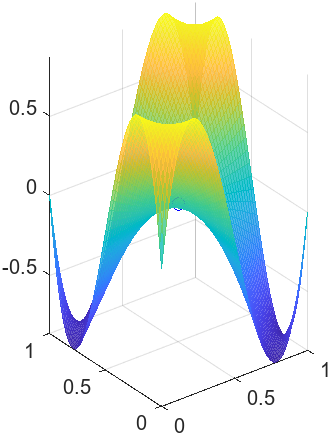
\includegraphics[height=0.35\textwidth]{sarokF.png}
	\hspace{5pt}
	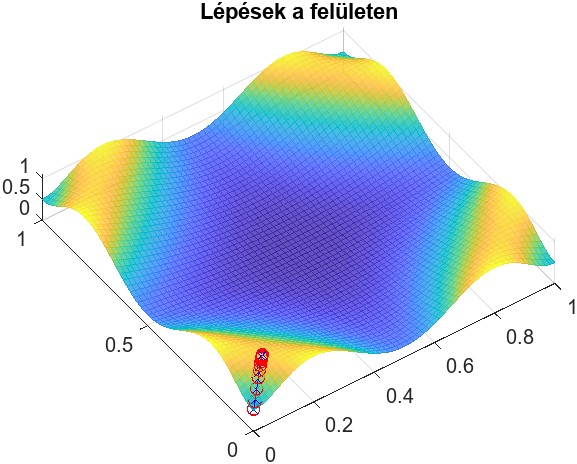
\includegraphics[height=0.35\textwidth]{sarokLep.png}
	\caption{Példa sarokpontok szükségességére}
	\label{fig:corners}
\end{figure}
A jobboldali ábrán a felület és az $(1/2,1/2,0)$ pont távolsága látható. Emellett a gradiens módszerek lépései szerepelnek az $(1/10,1/10)$ pontból indítva.

Ezen a példán az látszik, hogy a sarokpontokból el kell indítani a keresést, illetve hogy a felület belsejében lévő lokális minimumot nem lehet minden esetben a sarkokból megtalálni. Én ezért az $(1/2,1/2)$ pontot is hozzávettem a kiindulási pontokhoz.

\subsection{Oldalak}
Az alábbi példán az látszik, hogy a lokális minimum lehet az oldal mentén is, és azt nem feltétlenül találjuk meg a sarokpontból indulva.
\begin{figure}[H]
	\centering
	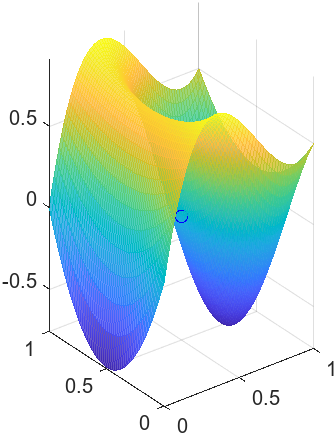
\includegraphics[height=0.3\textwidth]{oldalF.png}
\end{figure}
\begin{figure}[H]
	\centering
	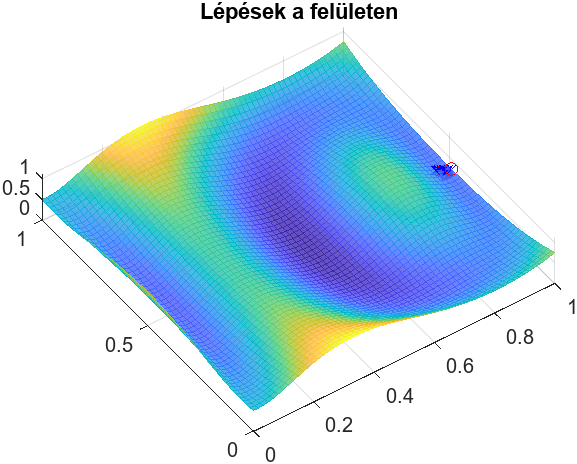
\includegraphics[height=0.35\textwidth]{oldalLep1.png}
	\hspace{5pt}
	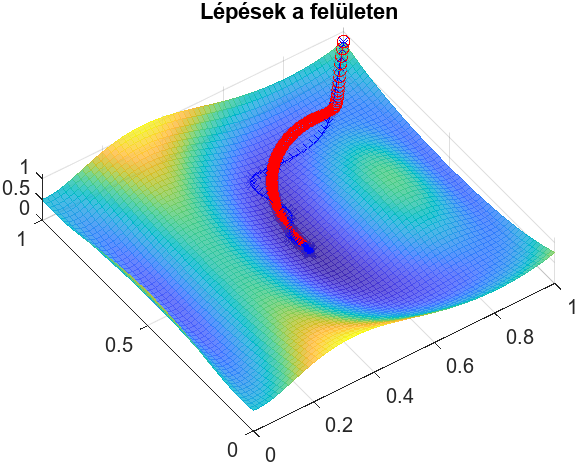
\includegraphics[height=0.35\textwidth]{oldalLep2.png}
	\caption{Példa oldalpontok szükségességére}
\end{figure}
Emiatt én az oldalak középpontját is hozzávettem a kiindulási pontokhoz.

\subsection{10 pont módszer}
$9$ indítási pont egy egyenletes $3\cross3$-as felosztás a paramétertérben. Ezzel a felület nagyobb vonásait lefedjük. Azért, hogy a módszer a felület közelében is gyorsan konvergáljon, a mintavételezési pont alatti felületi pontból is elindítom a keresést. Mivel grafikonon vagyunk, ez megegyezik az első két koordinátával.



\section{AdaMax algoritmus Bézier felületeken}
A 10 pont módszer helyességét szimulációval kívánom igazolni. Ehhez nagyszámú mintát generáltam, majd ellenőriztem, hogy a javasolt módszer minden alkalommal megtalálta-e a globális minimumot.

\subsection{Felületgenerálás}
A harmadfokú Bézier-felületek generálásához elég a $4\cross4$ kontrollpontot megadni. Ehhez egyenletes eloszlással véletlen pontokat vettem a $[-1,1]$ intervallumból. Az így keletkező felületek a közepükön meglehetősen laposak voltak. Ennek oka, hogy amíg a  $0.$ és a $3.$ harmadfokú Bernstein-polinom maximuma az $1$ értéket veszi fel, addig a középsők maximuma csak $4/9$. Ez különösen látványos a felület közepén, ott ugyanis két Bernstein-polinom szorzata áll melyek maximuma $(4/9)^2$. Ezen tulajdonság miatt a középső kontrollpontoknak sokkal kisebb hatása van, mint a szélsőknek, ahol ráadásul interpolál is a felület. Emiatt minden kontrollpont harmadik koordinátáját leosztottam a hozzá tartozó Bernstein-polinom maximumával.

\subsection{Mintavételezési pont generálás}
A mintavételezési pontokat a felület bennfoglaló dobozából és annak környezetéből vettem. Ehhez egy egyenletes felosztású térrács pontjait random vektorokkal eltoltam. Az ábrán egy példa merőleges vetülete látható.
\begin{figure}[H]
	\centering
	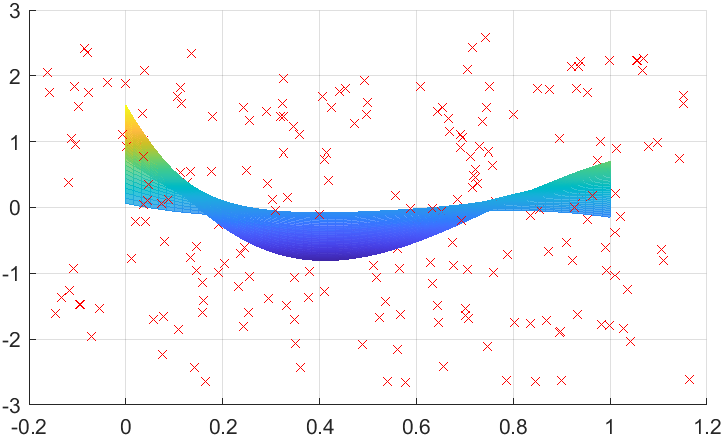
\includegraphics[width=0.5\textwidth]{mintavetel.png}
	\caption{Felület és ponthalmaz képe}
\end{figure}

\subsection{Referencia értékek}
Referencia értékként kiszámítottam minden mintavételezési pontra a ,,brute force'' módszer eredményét, azaz a távolságot egy $n\cross n$-es rácson kiértékeltem.
\begin{figure}[H]
	\centering
	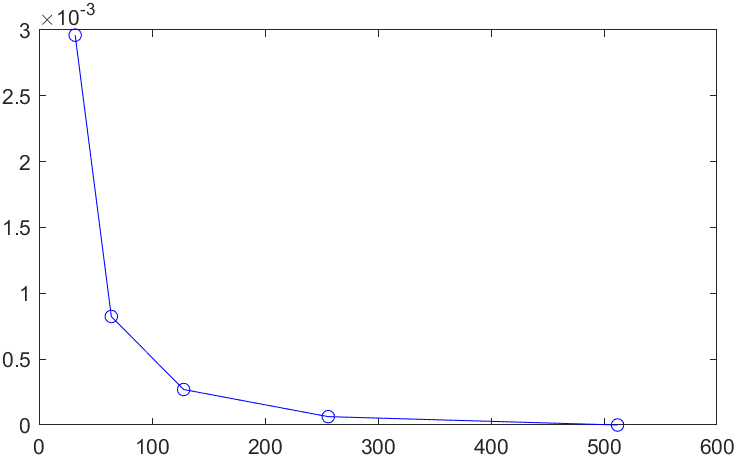
\includegraphics[width=0.5\textwidth]{ground_truth.png}
	\caption{Referencia érték maximális hibája a legnagyobb felbontáshoz képest}
\end{figure}
A tesztek alapján a hiba a műveletigénnyel arányosan csökken, pontosabban a felbontás ($n$) duplázásakor a hiba közel a negyedére csökken. A továbbiakban az $n=256$ értéket használom.



\section{Validáció}

A $10$ pontos algoritmust $1000$ különböző példára futtattam, majd összehasonlítottam a kapott miniumot a referencia értékkel. Mivel azt szeretnénk, hogy az algoritmus a \emph{legrosszabb} esetben is megadja az optimumot, azért a grafikonon az összes futtatás közül a relatív hiba maximumát ábrázoltam minden egyes lépésszámra.
\begin{figure}[H]
	\centering
	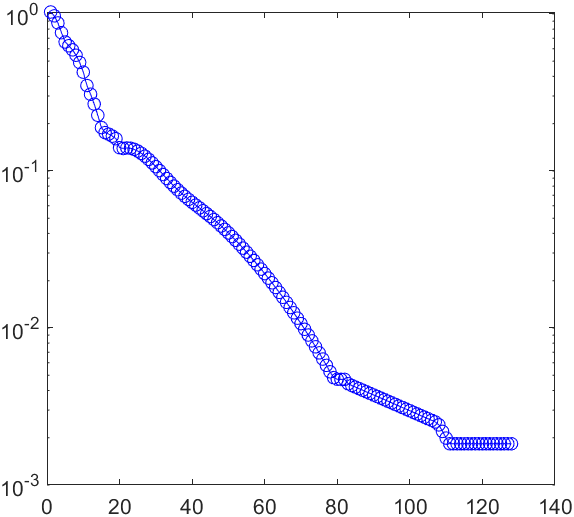
\includegraphics[width=0.5\textwidth]{stepcount.png}
	\caption{Abszolút hiba maximuma a lépésszám függvényében, logaritmikus skálán.}
\end{figure}
A módszer minden futtatás esetén megtalálta az optimumot legalább a referencia érték pontosságával, kevesebb, mint $120$ iteráció alatt. A grafikon $110$ lépés után azért laposodik el, mert az algoritmus eléri a refrencia érték pontosságát. Ha referenciának az utolsó iteráció által adott távolságot vesszük, akkor látható, hogy a módszer tovább konvergál.
\begin{figure}[H]
	\centering
	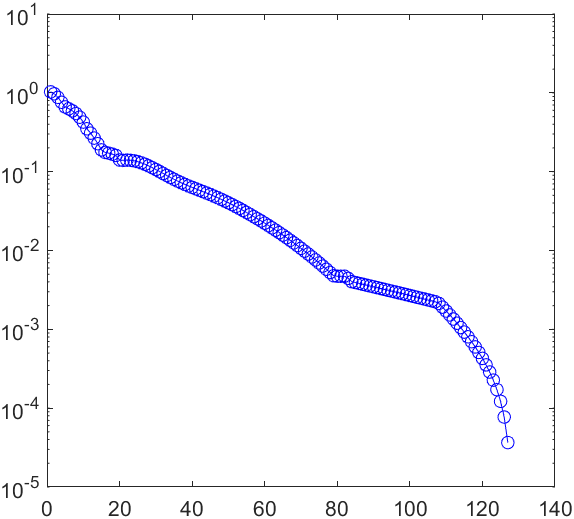
\includegraphics[width=0.5\textwidth]{005_8_99.png}
	\caption{Abszolút hiba maximuma az iteratív módszerhez viszonyítva.}
\end{figure}





% ------------------------------------------------------
\chapter{Implementáció}
\label{ch:impl}
% ------------------------------------------------------

Ebben a részben néhány fontos implementációs részletre térek ki. Ennek motivációja, hogy a CPU implementáció profilozásakor kiderült, az algoritmus az idő $60\%$-át a felület kiértékelésével és a gradiens kiszámításával tölti.

\section{de Casteljau algoritmus}
\subsection{Iterációval}
Az algoritmus CPU implementációja két egymásba ágyazott ciklussal működik. Ez \aref{lst:iter}-es forráskódban látható.

\begin{lstlisting}[caption={de Casteljau iterációval}, language={C++}, label={lst:iter}]
	float deCasteljou_iter(float4 pts, float t, float one_minus_t)
	{
		for (int j = 1; j <= 3; j++)
		{
			for (int i = 0; i <= 3 - j; i++)
			{
				pts[i] = one_minus_t * pts[i] + t * pts[i + 1];
			}
		}
		return pts[0];
	}
\end{lstlisting}

\subsection{Swizzle operátorokkal}
Részben azért esett a választás a köbös Bézier-felületekre, mert a GPU kód támogat műveleteket legfeljebb $4$ hosszú vektorokkal. Ez azt jelenti, hogy a felület kontrollponthálójának egy sora belefér egy ilyen vektorba. Az elméleti áttekintésnél láttuk, hogy a felület kiértékelése visszavezethető az egydimenziós problémára, így ezt a függvényt kell vektorizálni. Ezt a szintén hardveresen támogatott ú.n. swizzle operátorokkal tesszük. Ezek lényege, hogy a művelet elvégzése előtt a bemeneti vektorok elemeit tetszőlegesen átrendezhetjük, akár duplikálhatjuk is. A javított implementáció \aref{lst:swizzle}-es forráskódban látható.

\begin{lstlisting}[caption={de Casteljau swizzle operátorokkal}, language={C++}, label={lst:swizzle}]
	float deCasteljou_swizzle(float4 pts, float t, float one_minus_t)
	{
		for (int j = 1; j <= 3; j++)
		{
			pts.xyz = one_minus_t * pts.xyz + t * pts.yzw;
		}
		return pts[0];
	}
\end{lstlisting}

A programokat először a Radeon GPU Analyzer-rel hasonlítottam össze. A gépi kódban már egyáltalán nem lesz ciklus, mert a driver kibontja. A ciklusos implementációban 11, a swizzle implementációban 10 vektorművelet szerepelt. Ebből messzemenő következtetést nehéz levonni. A swizzle implementáció ciklusát kézzel is kibontottam. Ez nem okozott jelentős javulást. Végül lecseréltem minden sort egy lerp (lineáris interpoláció) utasításra. Az implementáció \aref{lst:lerp}-as forráskódban látható. Ezt a driver jobban tudja optimalizálni. 

\lstset{}
\begin{lstlisting}[caption={de Casteljau lerp függvénnyel}, language={C++}, label={lst:lerp}]
	float deCasteljou_lerp(float4 pts, float t)
	{
		pts.xyz = lerp(pts.xyz, pts.yzw, t);
		pts.xy = lerp(pts.xy, pts.yz, t);
		return lerp(pts.x, pts.y, t);
	}
\end{lstlisting}


\subsection{Mérési eredmények}
Az algoritmusokat a ,,Brute force'' távolságmező generáló módszer segítségével hasonlítottam össze, mert ez főként felületkiértékelést végez. Minden esetben egy $32^3$ méretű textúrát generáltam és kiátlagoltam $512$ futtatást. \Aref{tab:deCasteljau} és \ref{tab:deCasteljau2} táblázatok a számításhoz szükséges GPU-időt foglalják össze milliszekundumban. Először a Bézier-felületből készített magasságtérképet textúrába írtam, majd a távolságmező generálásakor onnan kiolvastam. \Aref{tab:deCasteljau} táblázat második oszlopában ezek az értékek szerepelnek. A harmadik oszlopban a távolságmező generálásakor számítottam ki a függvényértékeket.

Referenciának kimockoltam a de Casteljau függvényt azzal, hogy csak az utolsó sort hagytam meg. A GPU Analyzer-ből kiderül, hogy ekkor teljesen eltűnik a függvény, mert a driver mindenhol inline-olja. Ezt az értéket kivontam a harmadik oszlopból, így megkaptam, mekkora része a futási időnek a felület kiértékelése.

\begin{table}[H]
	\begin{center}
		\begin{tabular}{| c || c || c | c |}
			\hline
			(ms) & \textbf{Memóriából olvasva} & \textbf{Számítva} & \textbf{ebből de Casteljau} \\ 
			\hline\hline
			két ciklusos & 51,6 & 76,97	& 75,76 \\
			\hline
			swizzle	& 51,35	& 2,74 & 1,53 \\
			\hline
			kibontott & 51,33 & \textbf{2,63} & 1,42 \\
			\hline
			üres & 51,41 & 1,21	& 0 \\
			\hline
		\end{tabular}
	\end{center}
	\caption{de Casteljau algoritmus mérése egy $32^3$ méretű textúrán}
	\label{tab:deCasteljau}
\end{table}

A mérésekből kiderül, hogy a ciklusos implementáció nagyjából \emph{50-szer lassabb} GPU-n, mint a többi számításos verzió. A második oszlopban az értékek nagyjából megegyeznek, a futási idők pedig jóval a táblázatban szereplő legjobb idő felett vannak. Ebből arra következtethetünk, hogy ha memóriából olvassuk ki a felületértékeket, akkor a limitáció a memóriaelérés által okozott késleltetés lesz.

A legjobb megoldásokat összehasonlítottam egy nagyobb, $64^3$ méretű textúrán is. Ennek eredményeit \aref{tab:deCasteljau2} táblázat tartalmazza.

\begin{table}[H]
	\begin{center}
		\begin{tabular}{| c || c || c | c |}
			\hline
			(ms) & \textbf{Számítva} & \textbf{ebből de Casteljau} \\ 
			\hline\hline
			swizzle & 64,09 & 49,38 \\
			\hline
			kibontott & 62,13 & 47,42 \\
			\hline
			lerp & \textbf{52,85} & 38,14 \\
			\hline
			üres & 14,71 & 0 \\
			\hline
		\end{tabular}
	\end{center}
	\caption{de Casteljau algoritmus mérése egy $64^3$ méretű textúrán}
	\label{tab:deCasteljau2}
\end{table}

A kézzel kibontott ciklus nem okoz lényeges javulást, viszont a lineáris interpoláció nagyjából $25\%$-al gyorsabb. 


\subsection{Megjegyzések}
\begin{itemize}
	\item A felület kiértékeléséhez a kontrollpont-háló minden sorára meg kell hívni az algoritmust, majd az eredményekből álló vektorra megint. Ez összesen 5 de Casteljau függvényhívás.
	\item Matematikailag létezik ennél gyorsabb algoritmus, de nem használjuk, mert a numerikus stabilitásra nagyon oda kell figyelni GPU környezetben. (Szűk számábrázolás miatt.)
	\item Emellett az is megfigyelhető, hogy a matematikai műveletigény és a driver által generált kód futási ideje között nem feltétlenül intuitív az összefüggés.
\end{itemize}


\section{Pont-felület távolság és gradiense}

\subsection{Analitikus pont-felület távolság}
Legyen $E(e_1,e_2,e_3)$ a mintavételezési pont modell koordináta-rendszerben és $r(x,y) = (x,y,b(x,y))$ pedig a felület parametrikus egyenlete. Ekkor a távolság egy adott felületi és mintavételezési pontra:
$$ D_1(x,y) = \norm{E-r}_2 = \sqrt{(e_1-x)^2 + (e_2-y)^2 + (e_3-b(x,y))^2} $$
Ennek egyik parciális deriváltja: 
$$ \partial_xD_1 = \frac{2(x-e_1) + 2(b(x,y)-e_3)b_x(x,y)}{\sqrt{(e_1-x)^2 + (e_2-y)^2 + (e_3-b(x,y))^2}} $$
Ahol $b_x(x,y)$ a magasságfüggvény $x$ szerinti parciális deriváltja. A nevezőben lévő érték a távolság, ami a felület közelében $0$ közeli. Mivel a távolségfüggvényt a felülethez közel is kiértékeljük, ez mindenképp numerikusan instabil lesz, sőt, nullával osztást is eredményezhet. 

A távolságfüggvényhez a legközelebbi pontot akarjuk meghatározni a felületen. Mivel a négyzetgyök függvény szigorúan monoton nő, a norma négyzetének is ugyanott lesz minimum helye, ahol a normának.
$$ D(x,y) = \norm{E-r}_2^2 = (e_1-x)^2 + (e_2-y)^2 + (e_3-b(x,y))^2 $$
Ennek parciális deriváltjai: 
$$ \partial_xD = 2(x-e_1) + 2(b(x,y)-e_3)b_x(x,y) $$
$$ \partial_yD = 2(y-e_2) + 2(b(x,y)-e_3)b_y(x,y) $$
Ezt sokkal könnyebben és stabilabban tudjuk számolni.

\subsection{Gradiens számításának műveletigénye}
Távolságfüggvényeknél gyakori, hogy a gradienst szimmetrikus differencia módszerével határozzuk meg. Ehhez nem kell ismerni a távolságfüggvény képletét, csak ki kell értékelni több helyen. Egy kis $\varepsilon$ számot választva a gradiens közelítése: 
$$ b' \approx \frac{1}{2\varepsilon} \cdot \begin{pmatrix} b(x+\varepsilon,y) - b(x-\varepsilon,y) \\ b(x,y+\varepsilon) - b(x,y-\varepsilon) \end{pmatrix} $$
Itt a $b(x,y)$ függvény kiértékelését négyszer el kell végezni. Emellett egy kivonásra és egy szorzásra is szükség van. ($1/(2\varepsilon)$ konstans) Ez összesen 122 matematikai művelet. 

A parciális derivált számításához csak 12 mátrix elemet kell redukálni, így annak kiértékelése 22 matematikai művelet. $b$ totális deriváltjának analitikus számításához a két parciális deriváltat kell kiszámolni, ami 44 művelet. Mivel az utóbbi matematikailag hatékonyabb, ezt a verziót implementáltam.

\subsection{A távolság gradiense}
A totális derivált kifejezhető vektorokkal:
$$ D' = 2\left[\left(\begin{pmatrix} x \\ y \end{pmatrix} - \begin{pmatrix} e_1 \\ e_2  \end{pmatrix}\right)  + (b(x,y)-e_3)\cdot b'(x,y) \right]$$
Ezt a gradienst használjuk az iterációs módszerben. 


\section{AdaMax}
A AdaMax algoritmus kódja a pszeudokóddal teljesen ekvivalens. Kizárólag a numerikus stabilitásra kell figyelni. A vetített gradiens számításánál az $\varepsilon$ érték nem lehet túl kicsi. $\varepsilon = 10^{-6}$ érték például már a végeredményben is látható numerikus hibákat okoz. Én $\varepsilon = 10^{-4}$ értéket használtam.

Szintén numerikus hibák és a zéróosztás elkerülése végett a tapasztalati szórás minimumát is $10^{-4}$-re állítottam. Ezalapján $u$ frissítési szabálya: 
$$ u_t = \max (\beta_2 u_{t-1}, |g_t|, 10^{-4}) $$


